\documentclass{article}
\usepackage{listings}
\usepackage{graphicx} %插入图片的宏包
\usepackage{float} %设置图片浮动位置的宏包
\usepackage[space]{ctex}
\title{第一次实验}
\author{田鸿龙}
\date{\today}
\begin{document}
\maketitle
\section{Hello OS}
\subsection{运行截图}
\begin{figure}[H]
    \centering
    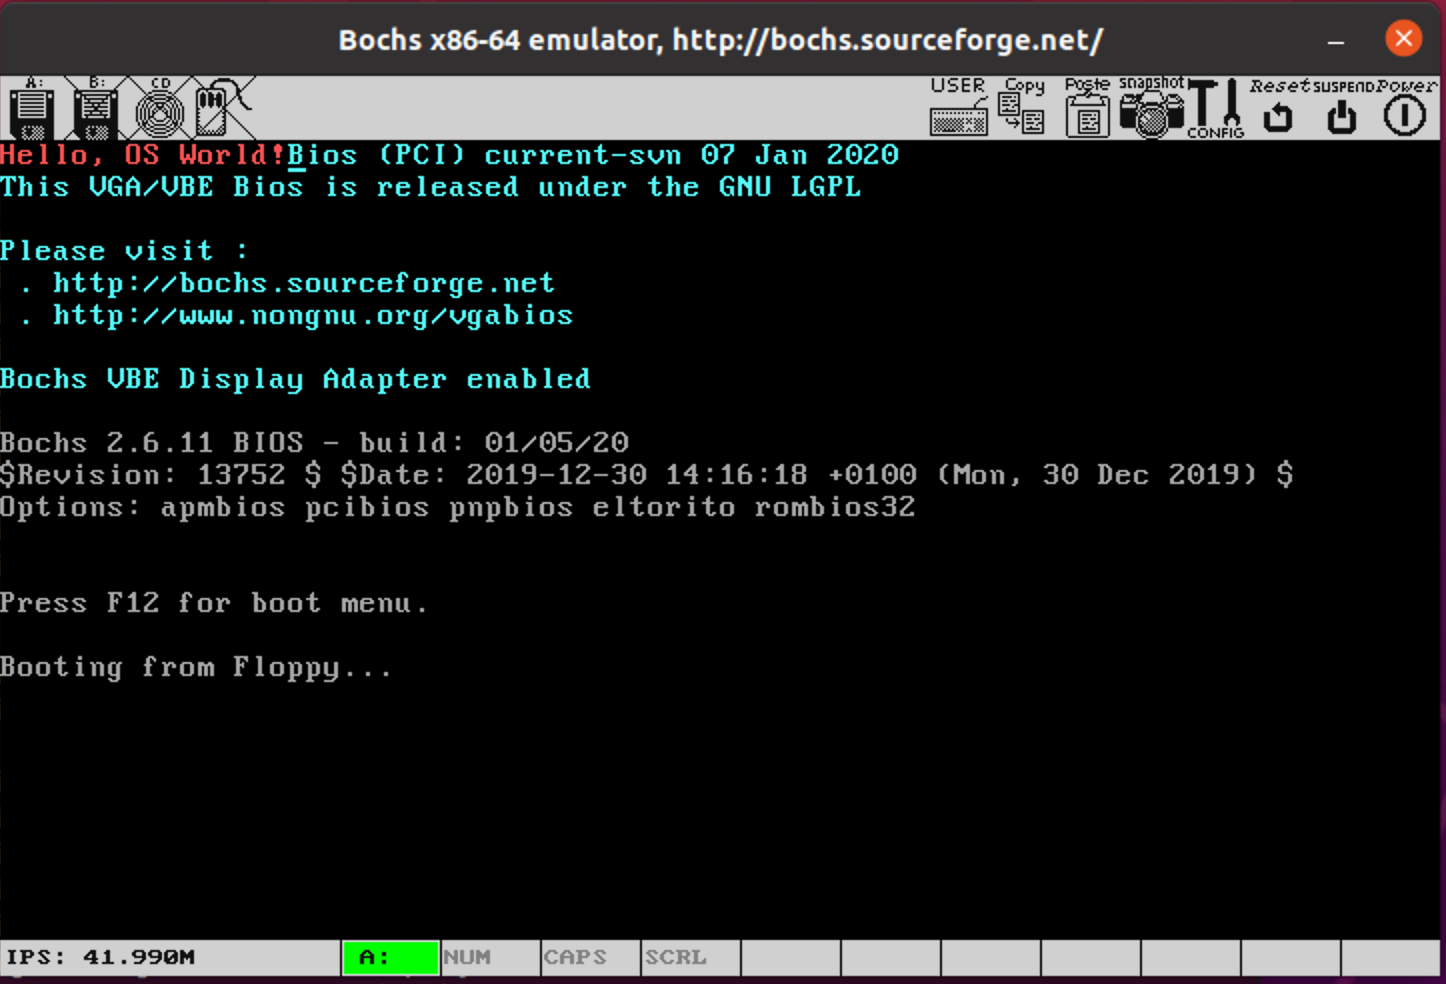
\includegraphics[width=0.7\textwidth]{bochs}
    \caption{bochs}
\end{figure}
\begin{figure}[H]
    \centering
    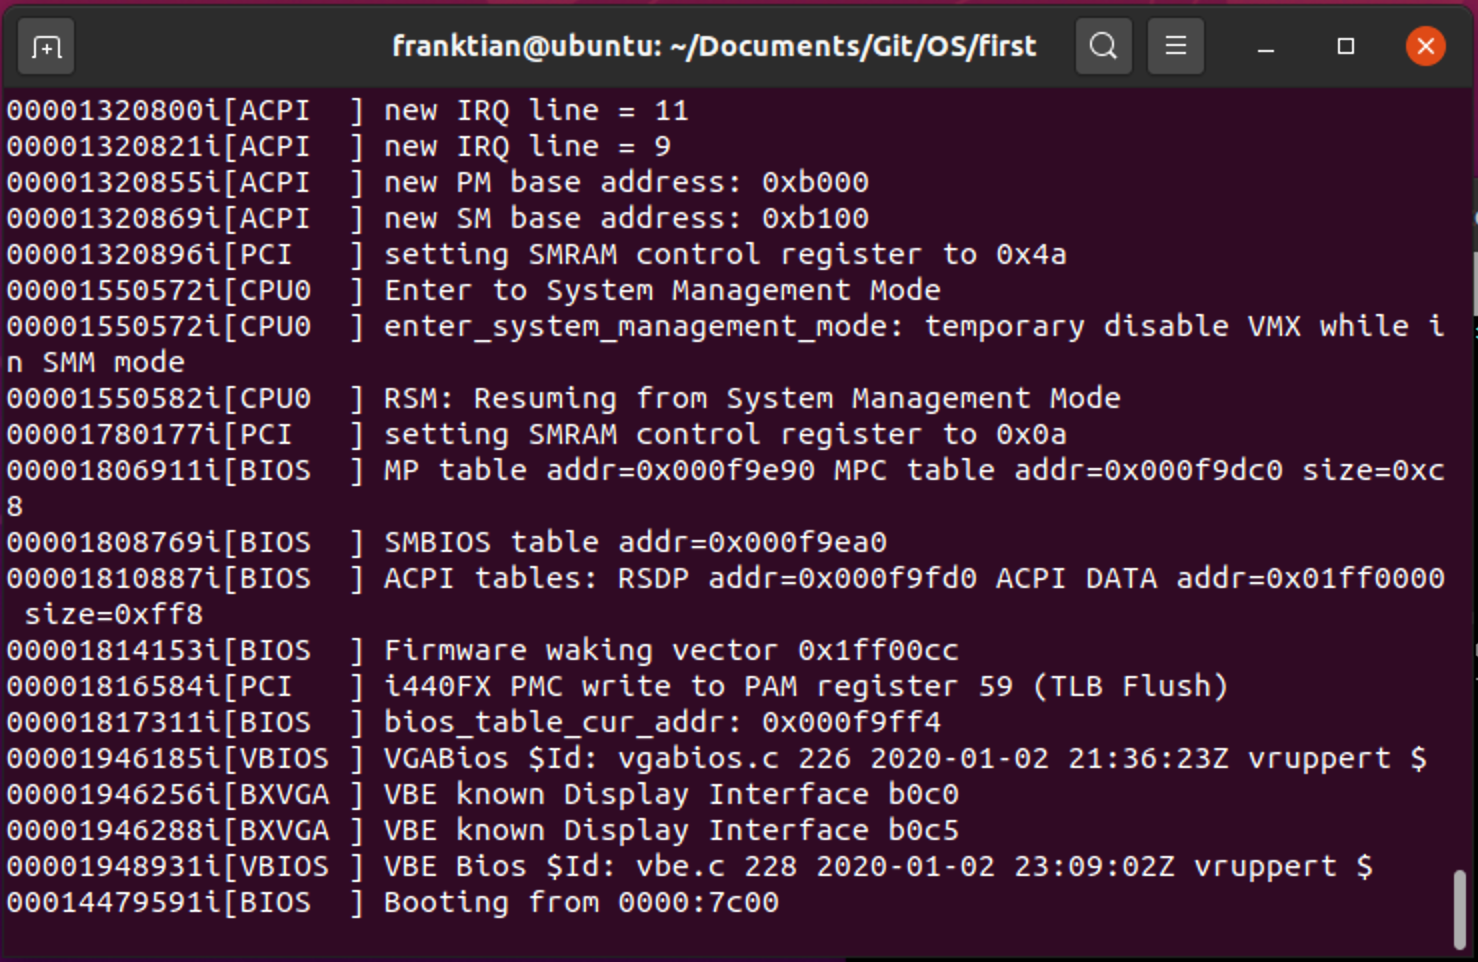
\includegraphics[width=0.7\textwidth]{terminal}
    \caption{terminal}
\end{figure}
\subsection{源代码}
\begin{lstlisting}
    org 07c00h
	mov ax, cs
	mov ds, ax
	mov es, ax
	call	DispStr
	jmp $
DispStr:
	mov ax, BootMessage
	mov bp, ax
	mov cx, 16
	mov ax, 01301h
	mov bx, 000ch
	mov dl, 0
	int 10h
	ret
BootMessage		db "Hello, OS World!"
times 510-($-$$)	db 0
dw 0xaa55
\end{lstlisting}
\section{汇编语言实践}

\section{问题清单}
\subsection{请简述 80x86 系列的发展历史}
\subsection{说明小端和大端的区别,并说明 80x86 系列采用了哪种方式?}
\subsection{8086 有哪五类寄存器,请分别举例说明其作用?}
\subsection{什么是寻址?立即寻址和直接寻址的区别是什么?}
\subsection{请举例说明寄存器间接寻址、寄存器相对寻址、基址加变址寻址、相对基址加变址寻址四种方式的区别}
\subsection{请分别简述 MOV 指令和 LEA 指令的用法和作用?}
\subsection{请说出主程序与子程序之间至少三种参数传递方式}
\subsection{如何处理输入和输出,代码中哪里体现出来?}
\subsection{有哪些段寄存器}
\subsection{通过什么寄存器保存前一次的运算结果,在代码中哪里体现出来。}
\subsection{解释 boot.asm 文件中,org 0700h 的作用}
\subsection{boot.bin 应该放在软盘的哪一个扇区?为什么?}
\subsection{loader 的作用有哪些?}
\subsection{解释 NASM 语言中 [ ] 的作用}
\subsection{解释语句 times 510-(\$-\$\$) db 0,为什么是 510? \$ 和 \$\$ 分别表示什么?}
\$表示当前地址

\$\$表示当前段的地址
\subsection{解释配置文件 bochsrc 文件中各参数的含义}
\begin{lstlisting}
megs:32
display_library: sdl
floppya: 1_44=a.img, status=inserted 
boot: floppy
\end{lstlisting}

\end{document}
